\chapter{Trijunction of Majorana nanowires}

In this chapter we demonstrate that the coupling of three pairs of MBS in a trijuction is determined by the geometrical details of the central semiconducting cavity.
For certain geometrical configurations, a MBS pair couples resonantly with successive cavity states as in the so-called \textit{resonant trapping}, while in other cases the coupling is mediated by individual non-overlapping levels.

We simulate the pair coupling of three Majorana nanowires mediated by a semiconducting cavity using Kwant.
For each experiment, a pair of nanowires is set to host MBS in each sub band while the other nanowire is fully depleted.
We consider the strong coupling regime where there are no tunnel barriers between the cavity and the nanowires.
Furthermore, the phase difference between the selected nanowires is tuned such that the coupling is at a maximum.
\textit{The coupling energy of each pair is extracted as the value of the lowest non-zero eigenvalue with respect to the cavity chemical potential}.

The cavity chemical potential is varied in a range of $4$ meV around the first resonance for all cavities.
In this range, there are multiple levels that couple resonantly with a given pair of MBS.
\textit{In order to characterise the coupling, we extract the highest resonance peak for each geometry.}
Then, we classify them according to their operational robustness, that is, height and width.

\section{Quasi-one dimensional cavities}

\begin{figure}[h!]
\centering
  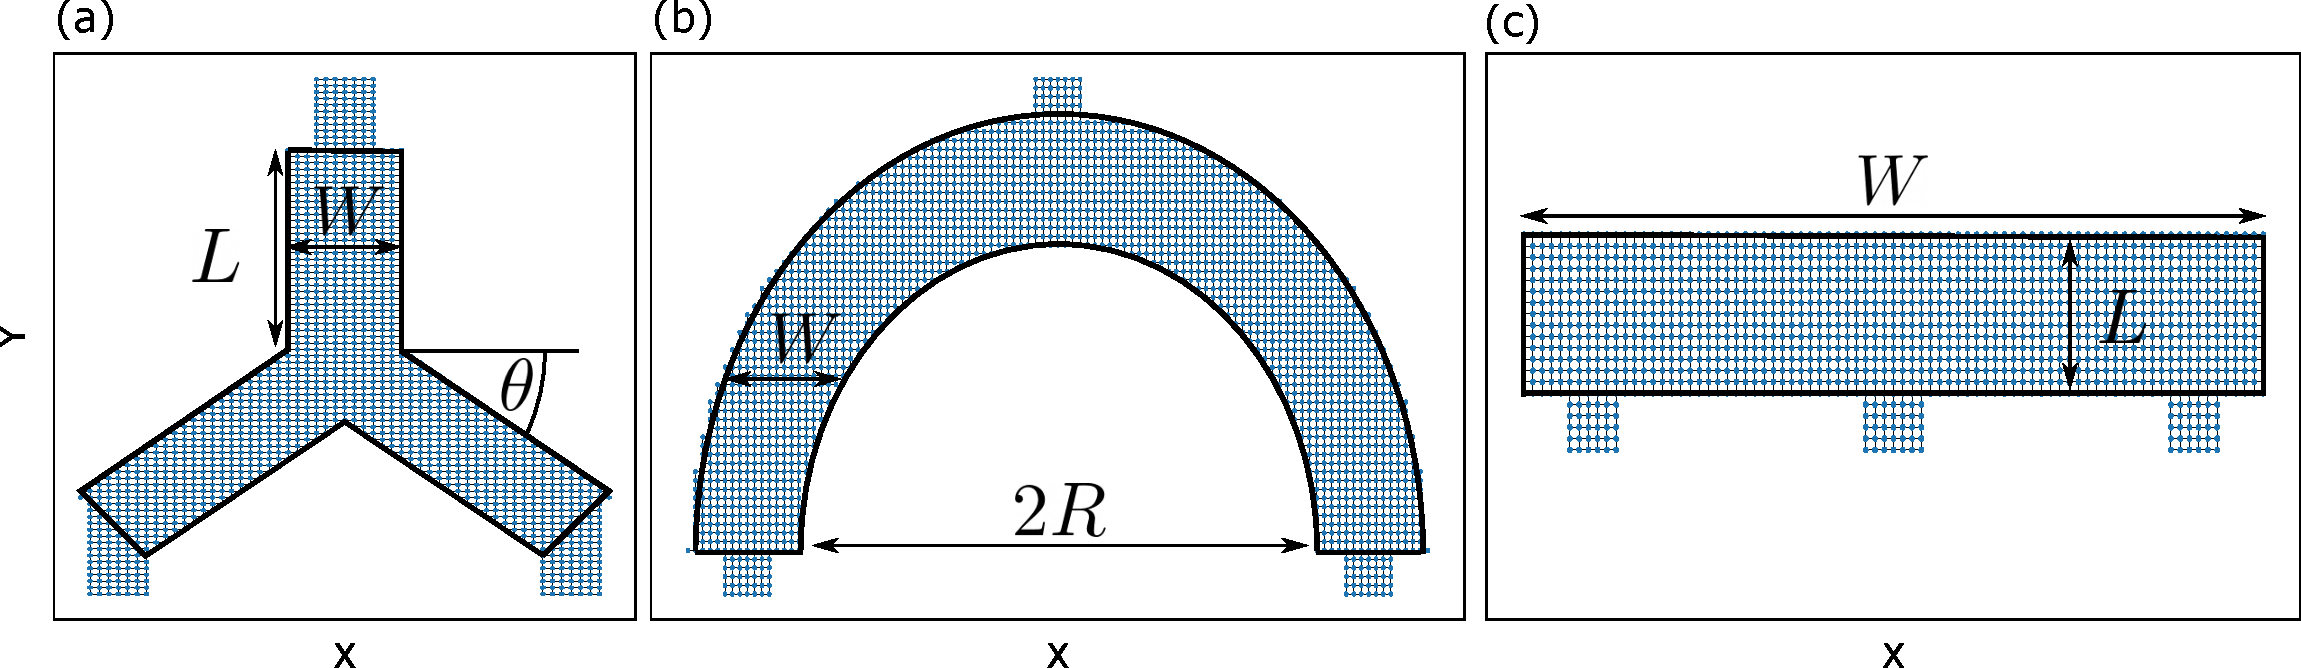
\includegraphics[width=0.9\linewidth]{figures/1d_cavities.pdf}
  \caption{Kwant systems describing the three quasi-1D cavities: (a) Y-shaped defined by three parameters: arms length and width, $L$ and $W$, and lateral arms angle $\theta$. (b) Half-ring defined by the radius $R$ and the width $W$. (c) Rectangular stripe defined by the length $L$ and width $W$.}
  \label{fig:1d}
\end{figure}

Let us start by building the simplest possible Majorana trijunction.
Consider a quasi-1D cavity with mirror symmetry along the $y$-axis.
Then, the position of the three nanowires is fixed: one is attached at the center, and one at each end.
Consequently, the phase shift for the central MBS pairs is symmetric around $\pi$.
Similarly, the coupling of the left-center MBS pair and center-right MBS pair is the same.
Under these constrains, we study how the geometry affects the coupling of the two different pairs.

We consider three cavity geometries:
In Fig. \ref{fig:1d} (a) one can observe a Y-shaped cavity. 
In Fig. \ref{fig:1d} (b) one can observe a half-ring stripe cavity with three nanowires attached in a fork-like geometry. 
In Fig. \ref{fig:1d} (c) one can observe a rectangular stripe cavity with three Majorana nanowires attached.

It is a challenge to build a trijunction that reliably and selectively couples all three pairs of MBS.
It is straightforward to couple a single MBS pair in a quasi-1D geometry since the left and right MBS pair will fully enclose the cavity wavefunctions.
However, it is a challenge to create a system where the remaining two pairs can couple in a similar way.

\subsection{Size dependence}

Initially, the overall size of the system is varied, and a transition from the small to the long junction regime is found for all geometries.
In Fig. \ref{fig:1d_results} one can observe the evolution of the largest resonance peak for each geometry as a function of the system size.

\begin{figure}[h!]
\centering
  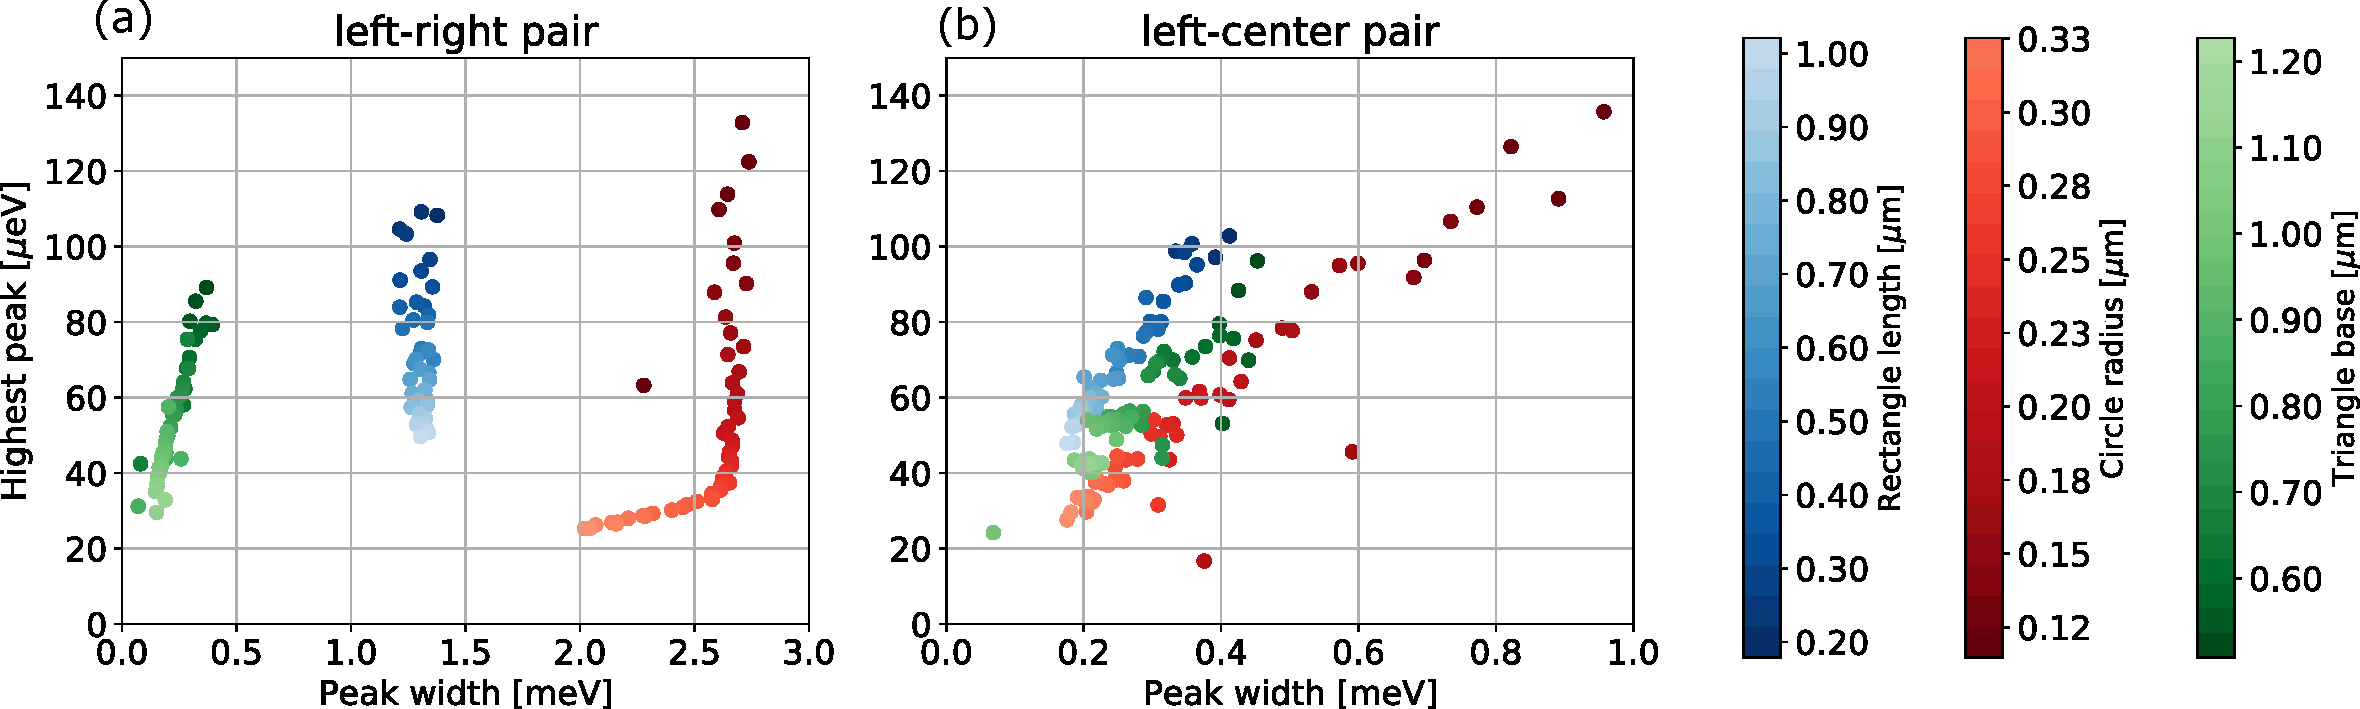
\includegraphics[width=\linewidth]{figures/couplings_1d.pdf}
  \caption{Geometrical dependence of the resonant coupling peaks for three quasi-1D geometries that correspond to each colorbar. The system was tuned to the lowest Majorana band. (a) Left-right MBS pair coupling. (b) Left-center MBS pair coupling.}
  \label{fig:1d_results}
\end{figure}

The coupling of the left and right MBS pair shows a clear geometrical dependence as can be observed in Fig. \ref{fig:1d_results} (a).
Each geometry occupies a separate region in the resonant height-width plane.
The ring cavity has the most robust resonant peaks.
For small $R$, the coupling is larger than any other geometry, and it is close to $\Delta/2$.
Similarly, the width is the largest, and it persists even for rings with diameter $1$ $\mu$m after which decays.
Then follows the stripe geometry that has approximately the same width for all considered widths.
Finally, the Y-shaped cavity has overall the smallest resonant peak width. 

The coupling of the central MBS pairs, on the contrary, cannot be easily separated for each geometry.
Generally, one can see three diagonal stripes in Fig. \ref{fig:1d_results} (b) where the stripe geometry has the largest resonant peak height.
The peak width decreases as the size increase, and it has the same slope for all geometries.
Nevertheless, for sufficiently small sizes, the ring geometry has peak heights and widths larger than any other geometry.

\subsection{Resonant trapping}

\begin{figure}[h!]
\centering
  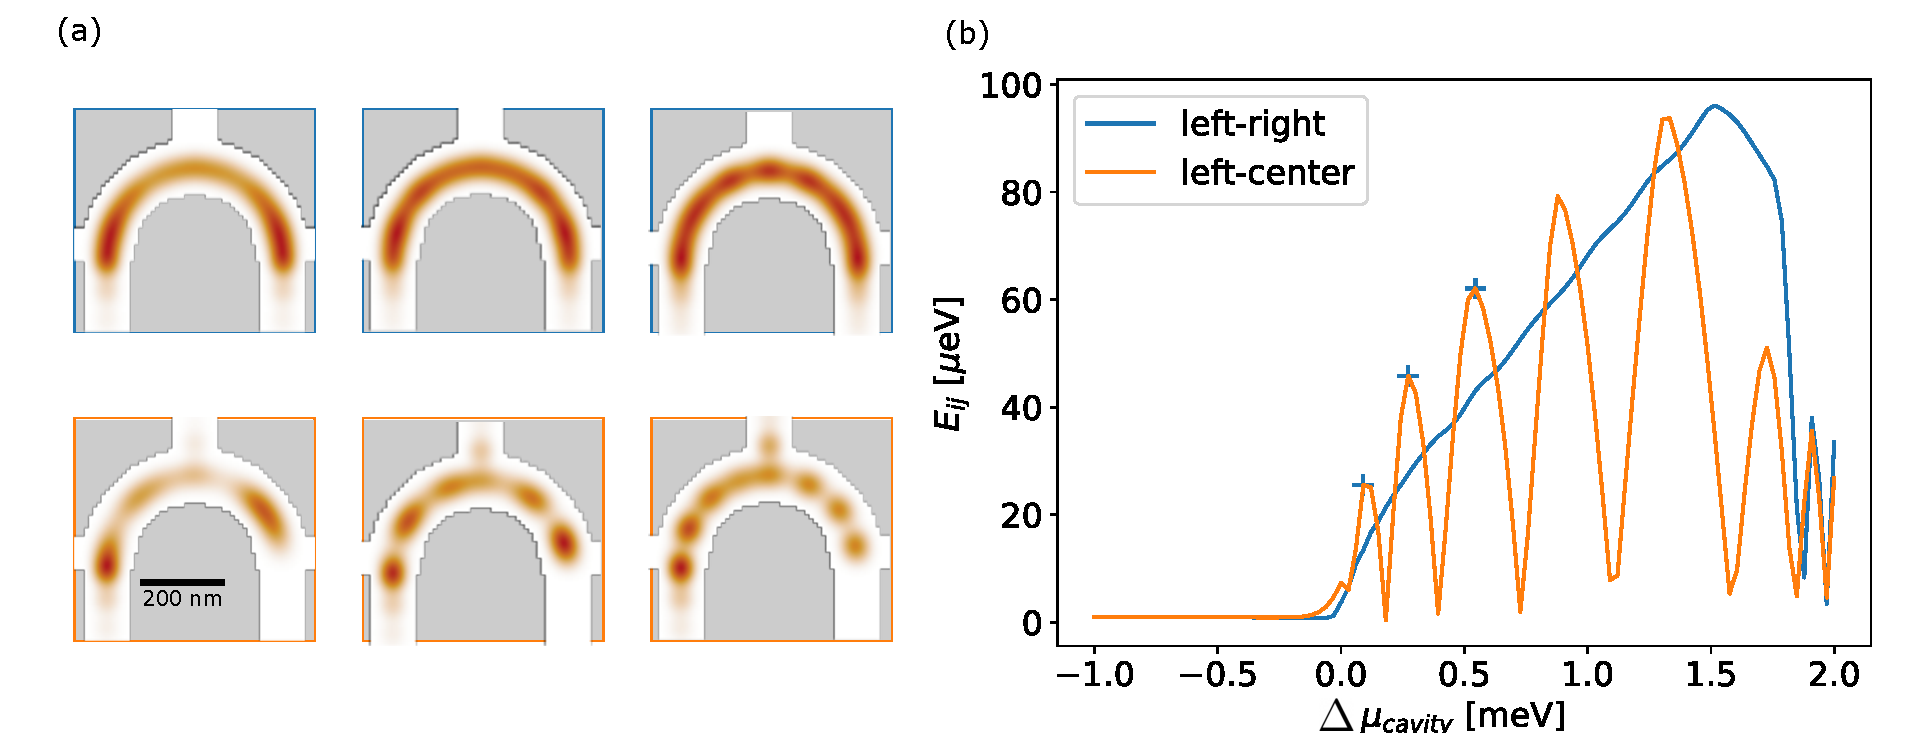
\includegraphics[width=\linewidth]{figures/resonant_trapping_ring.pdf}
  \caption{Spectra for a half-ring shaped cavity of width $W=110$ [nm] and radius $R=300$ [nm]. The system was tuned to the lowest Majorana band. (a) Coupling of each MBS pair. Center-right pair is the same curve as left-center pair. Crosses indicate the positions at where the wavefunction (b) are taken. The color of the frame in (b) corresponds each MBS pair in (a).}
  \label{fig:resonant_trapping}
\end{figure}

Let us consider the half-ring cavity.
When the left and right nanowires are close to the ends of the cavity, the MBS pair couple along a sequence of overlapping resonant states as can be seen in the blue line of Fig. \ref{fig:resonant_trapping} (a).
\textit{The cavity states interfere constructively and the coupling accumulates creating a single wide peak over the resonant region.}
It depends crucially on having the lead states around all of the cavity wavefunction as can be seen in Fig. \ref{fig:resonant_trapping} (b).
This phenomena is known as \textit{resonant trapping}.

\textit{For the central pairs coupling, in contrast, a band of resonances cannot form since the cavity wavefunction is not fully enclosed.}
When coupling the left and central MBS, the cavity region close to the right lead acts as a particle in a box with multiple individual levels that repel each other.
Consequently, we observe the orange line shown in Fig. \ref{fig:resonant_trapping} (a) where the resonant band is divided in individual resonances.

The difference when coupling multiple MBS pairs relies on the geometric configuration of the cavity wavefunctions and the MBS relative positions.
\textit{Then, one can explain the distribution of couplings observed in Fig. \ref{fig:1d_results}.}
The left and right MBS in the ring and stripe geometry have an approximately constant and large widths over the different system sizes because cavity levels remain resonant.
On the other hand, the coupling of the central MBS pairs in any geometry has a much smaller width because some part of the wavefunction is not coupled.
Particularly, the Y-shaped junction has a small width for all pairs because no resonant trajectories can be created in such geometry.

\section{Two dimensional cavities}

\begin{figure}[h!]
\centering
  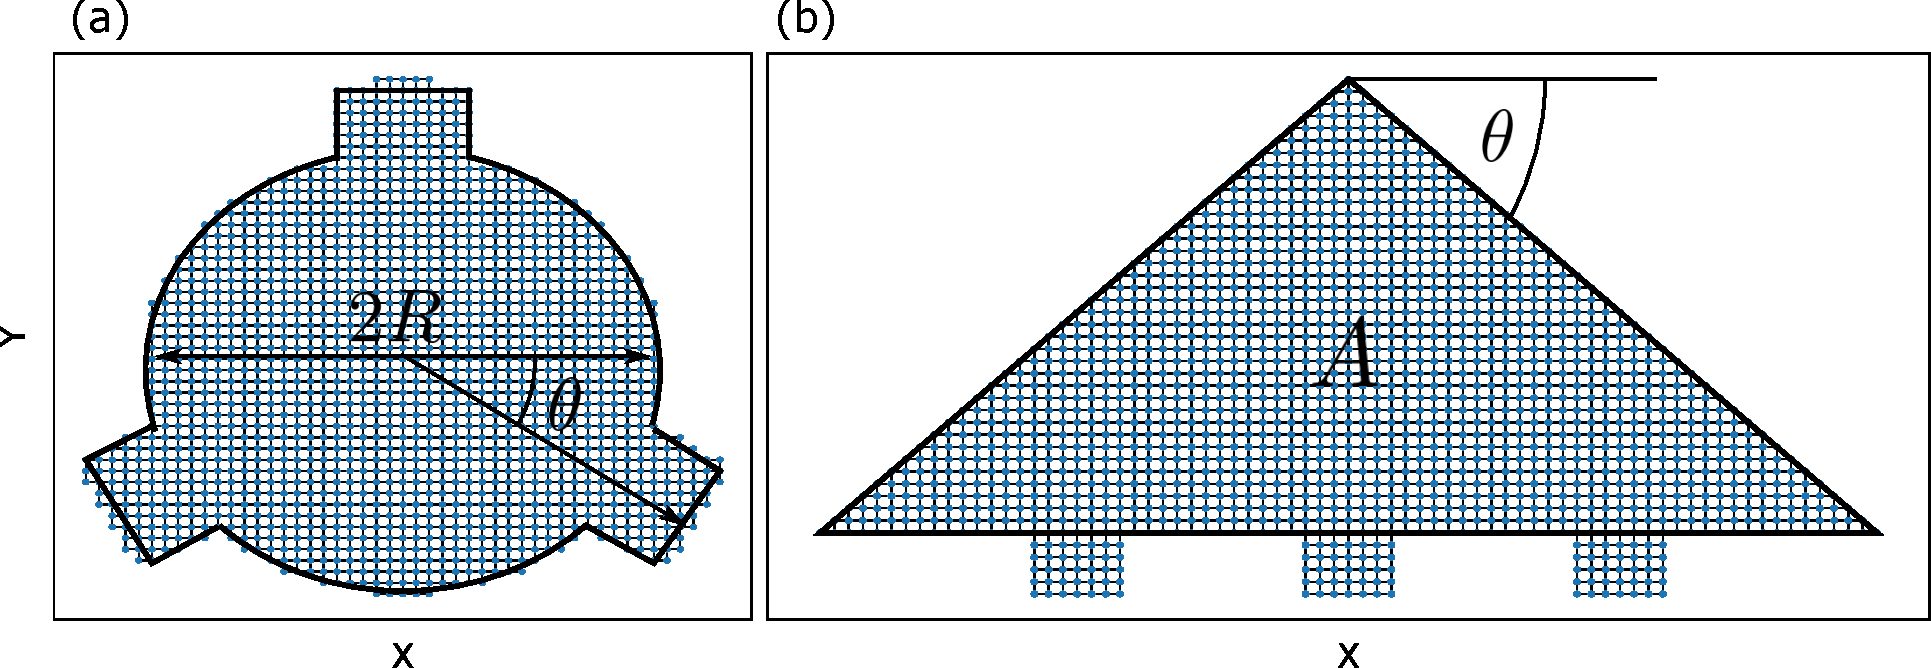
\includegraphics[width=0.9\linewidth]{figures/2d_cavities.pdf}
  \caption{Left: Kwant system of a half-ring shaped cavity. It is defined by the radius $R$ and the width $W$. Thiner rectangular segments represent the positions of the Majorana nanowires attached. Right: Lowest four eigenstates of the cavity with the nanowires fully depleted.}
  \label{fig:2d}
\end{figure}

\textit{In a ballistic cavity, the motion of the electrons is determined by the shape of the cavity and leads.}
The electrons follow semiclassical trajectories connecting different leads that can be identified as peaks in the conductance.
Following such intuition, we explore if changes in the geometry of a 2D cavity can be used to modulate the coupling of different MBS pairs.
Particularly, we explore how the angular dependence of the incoming modes, and internal angles of the cavity, influence the MBS coupling.

We consider three geometries:
In Fig. \ref{fig:2d} (a) one can observe a circular cavity with Majorana nanowires attached in a fork-like geometry.
In this geometry one can control the angle of the incoming MBS.
In Fig. \ref{fig:2d} (b) one can observe a triangular cavity with nanowires attached at the lower side.
In this geometry one can control the angle of MBS scattering within the cavity by changing the diagonal sides.
In order to explore to role of the positioning of the leads, we explore a variation of the triangular geometry with the central lead in the top side.
Lastly, we consider a rectangular geometry that can be created by extending the length of the stripe geometry shown in Fig. \ref{fig:1d} (c).

\subsection{Size dependence}

Let us start by discussing the size dependence of the cavities.
In Fig. \ref{fig:2d_size_results} one can observe the size dependence of the resonant peak for the three two-dimensional geometries.

\begin{figure}[h!]
\centering
  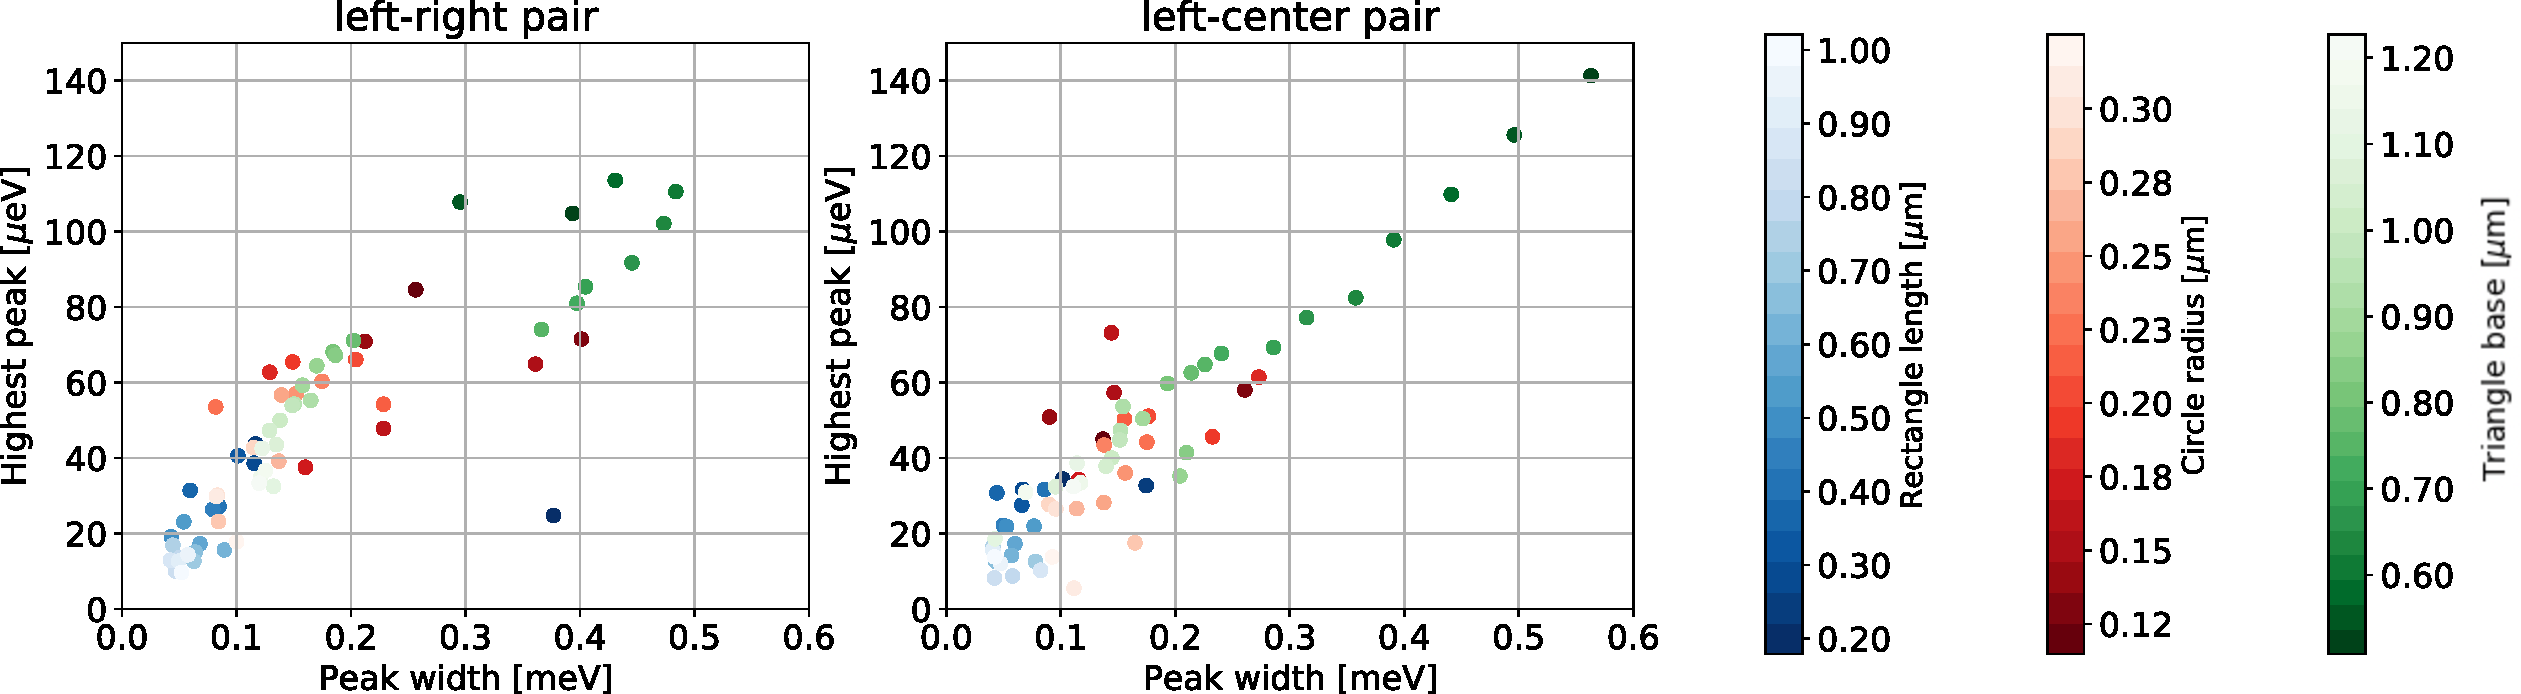
\includegraphics[width=\linewidth]{figures/couplings_2d.pdf}
  \caption{Size dependence of the three 2D geometries considered in this section corresponding to each colorbar. The system was tuned to the lowest Majorana band. The (a) left right and (b) left center largest resonant peaks are shown. The angle of all the cavities here is $\theta=\pi/4$.}
  \label{fig:2d_size_results}
\end{figure}

Overall, there is no major distinction between the coupling of different pairs.
All couplings decays as the system size increases following a diagonal line in panels (a) and (b).
Nevertheless, the geometry dependence can be seen in three different regions along the diagonal.

On the rightmost region, one observes that the triangular geometry has the largest couplings and widths for small sizes.
Descending along the diagonal, the triangular and circular geometries overlap.
Remarkably, there is a significant size difference between them in the overlapping region, approximately $500$ nm.
Most of circular geometries are concentrated in this region.
At the bottom of the diagonal, one observes that the worst MBS couplings happen for rectangular geometries.

\subsection{Angular dependence}

The angle is changed in two triangular cavities, one circular cavity, and the Y-shaped cavity.
The resulting coupling for each pair and geometry is shown in Fig. \ref{fig:angles_couplings}.

\begin{figure}[h!]
\centering
  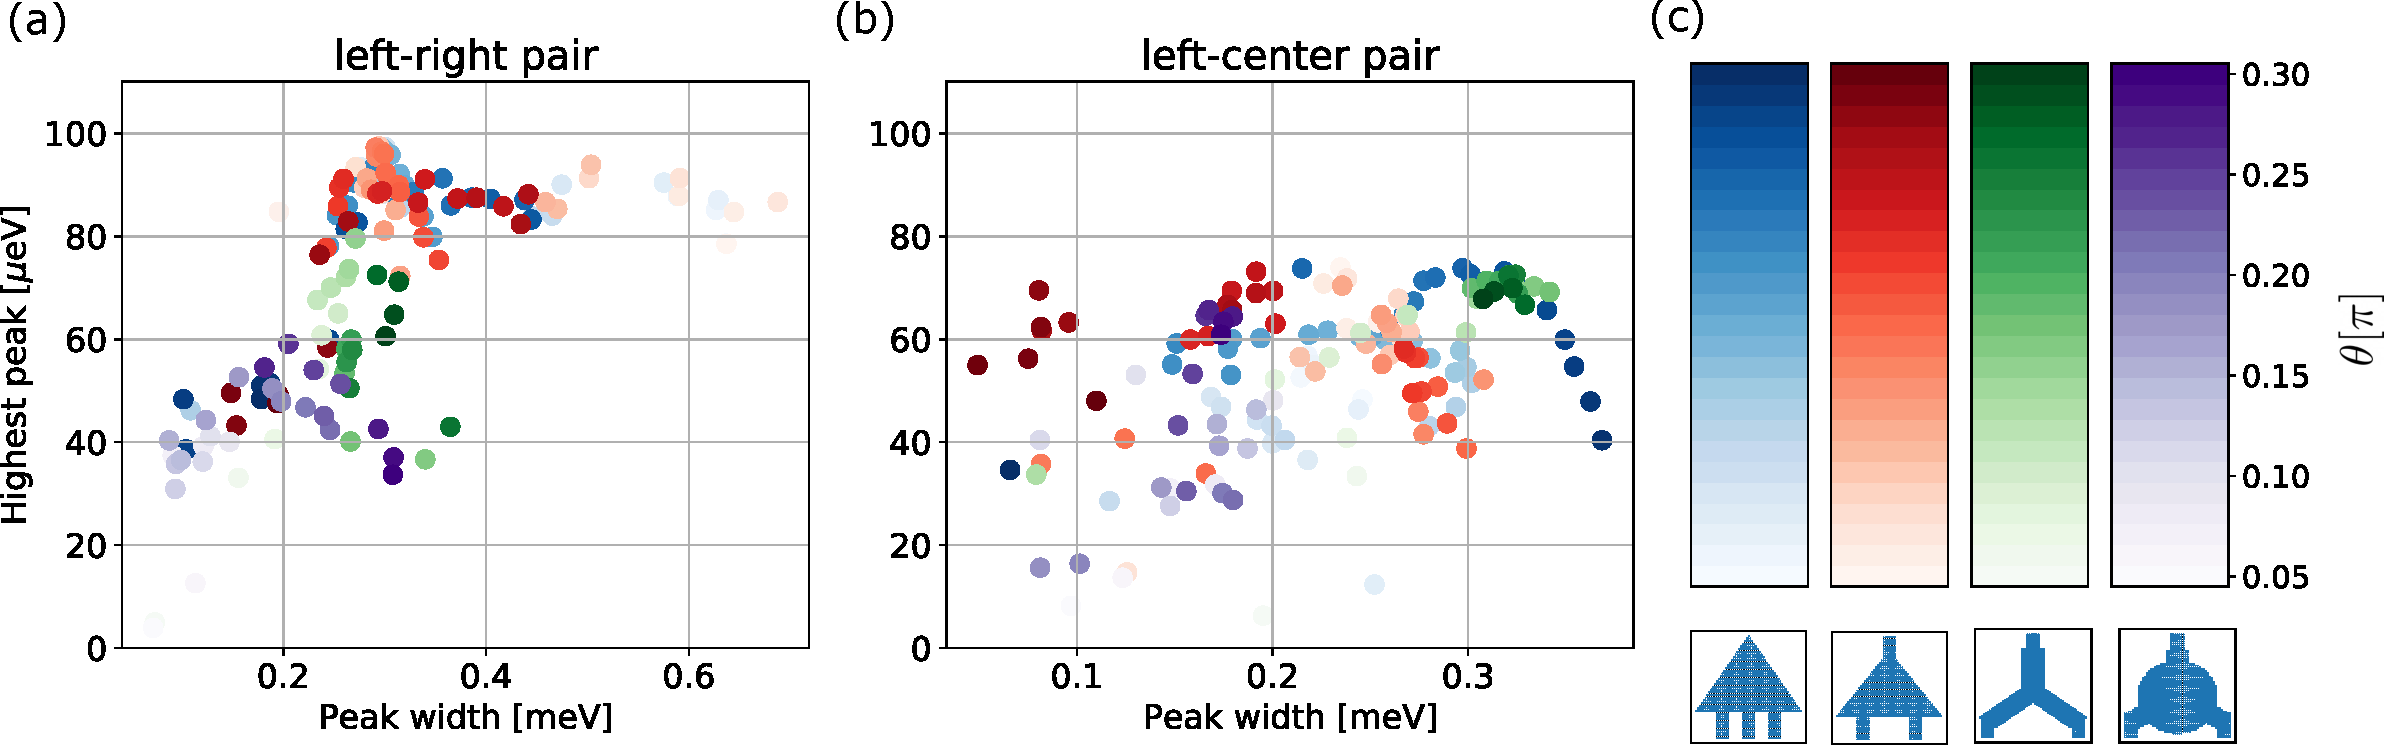
\includegraphics[width=\linewidth]{figures/couplings_angles.pdf}
  \caption{Angular dependence of the resonant coupling peaks for four geometries with angle dependence. The system was tuned to the lowest Majorana band.  Each one corresponds to a colorbar as depicted in (c). (a) Left-right MBS pair coupling. (b) Left-center MBS pair coupling. The area of the triangular cavities was $A=900$ $[a^2]$. The radius of the circular cavity is $R=250$ [nm]. The size of the Y-shaped cavity is similar to that of the triangular cavity.}
  \label{fig:angles_couplings}
\end{figure}

The triangular geometry shows a transition from the resonant trapping regime to the single resonance regime while maintaining an approximately constant peak height.
One can observe that the peak height stays around the same value for a large range of angles in panel (a).
This behaviour is present in both triangular geometries since the red and blue dots highly overlap.
The width, on the other hand, is inversely proportional to the angle.
For small angles, the width is the largest for 2D geometries, around $0.7$ meV.
As the angle increase, the width decreases until it saturates around $0.3$ meV.

In order to understand this behaviour, let us observe that for small angles the triangular cavity resembles a quasi-1D system.
By cutting the edges of the stripe geometry, the wavefunction is concentrated towards the center such that it can be easily trapped between the left and right leads as observed in the blue curve of Fig. \ref{fig:triangle_transition} (a).
As the angle increases, the resonant band splits into several sub bands that contain a few resonances each as observed in Fig. \ref{fig:triangle_transition} (b).
If the angle increases further, these resonances fully split into individual levels, thus explaining the saturation found in Fig. \ref{fig:angles_couplings} (a).

The coupling of the left and central MBS pair -on the contrary- is more complicated to analyse due to the high overlap between geometries as observed in Fig. \ref{fig:angles_couplings} (b).
Couplings for both triangular geometries are around the same region in width and height for small angles.
As the angle increases, the width of the configuration with central lead at the lower side (blue) increases, while the other configuration (red) decreases.

It is remarkable that the triangular geometry has two configurations that can be used to operate a Majorana trijunction with similar coupling magnitude and width for all MBS pairs.
These two configurations are shown in Fig. \ref{fig:triangle_transition}.
Note, however, that the small angle configuration would be rather considered a quasi-1D system since the ration between its dimensions.
That is the reason why the resonant band has such a large width and encloses many states.
Nevertheless, resonant trapping is still present in the second configuration, but with fewer states inside the resonant band.

\begin{figure}[h!]
\centering
  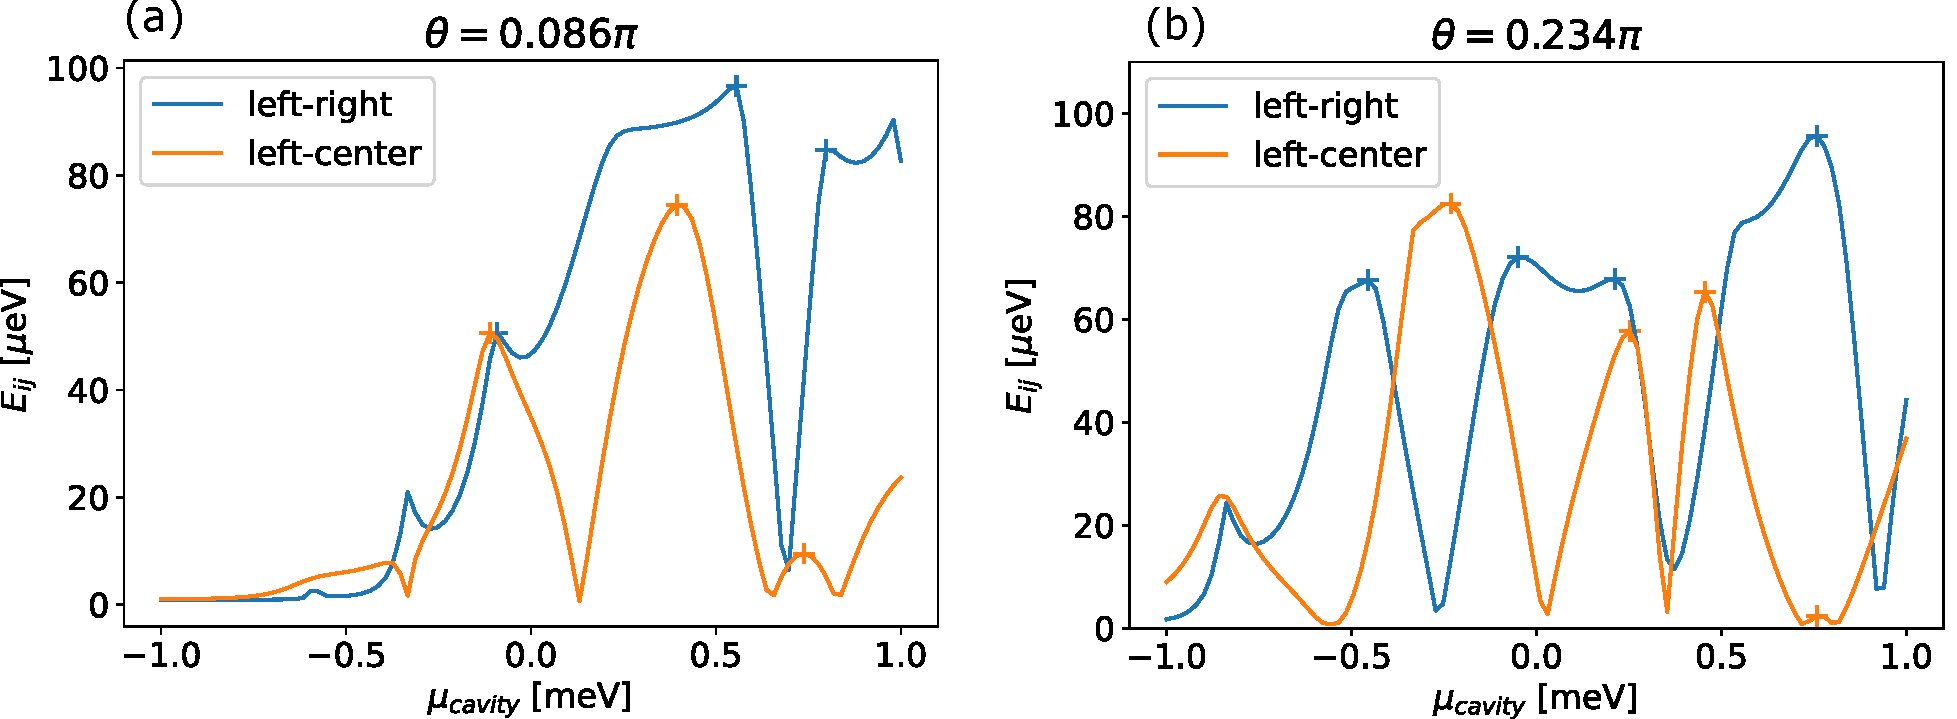
\includegraphics[width=0.8\linewidth]{figures/triangle_couplings.pdf}
  \caption{Coupling of triangular geometries with the central lead at the (a) top and (b) bottom sides. The total area of the triangle is $A=1200$ $[a^2]$.}
  \label{fig:triangle_transition}
\end{figure}

For the remaining geometries, there is indeed a modulation for the left and right MBS pairs.
However, the overall coupling remains smaller and narrower than the triangular case.
Interestingly, the left and central MBS coupling for the Y-shaped cavity converges to a region around $(0.3 meV, 70 \mu eV)$ as the angle increases (see Fig. \ref{fig:angles_couplings} (b) green points).
On the other hand, the behaviour of this pair in the circular cavity does not show a clear trend.

\subsection{Majorana sub bands}

By tuning each nanowire sub band into the topological phase, we probe the momentum distribution of the cavity states.
In Fig. \ref{fig:sub_bands} one can observe the mean coupling for each band.
It has been averaged over all geometrical configurations and all MBS pairs since no clear distinction between them was found.

\begin{figure}[h!]
\centering
  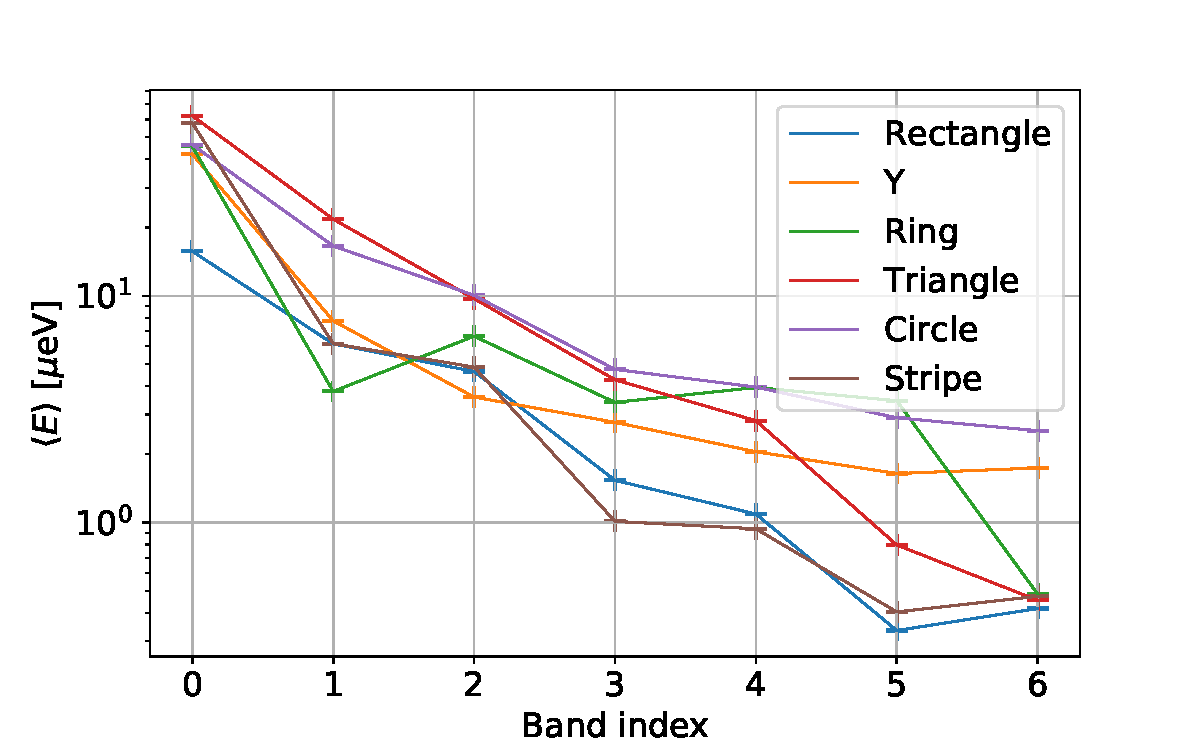
\includegraphics[width=0.6\linewidth]{figures/sub_bands_results.pdf}
  \caption{Mean geometry-pair coupling for all Majorana sub band and all geometries considered in this section. The geometry average was taken over the data shown in Fig. \ref{fig:2d_size_results}.}
  \label{fig:sub_bands}
\end{figure}

\textit{Overall, the coupling decays exponentially as the band index increases.}
The decay is modulated by the geometry, but the trend holds in all cases.
There is, approximately, two order of magnitude decrease in the coupling from the lowest to the highest band.

\textit{The lowest band carries the largest coupling.}
This allows us to infer that the momentum distribution of cavity states is dominated by low momentum states.
This is reasonable since the coupling of spatially separated MBS requires delocalised cavity states.
However, a precise quantitative description of the momentum profiles inside the cavity goes beyond the scope of this work.